\chapter{Group Learning: A Collective Knowledge Distillation Solution for Domain Transfer in Fact Verification \label{chapter:emnlp2021}}


Neural networks have achieved state-of-the-art performance across many natural language processing (NLP) tasks, usually in supervised settings.
However, as shown before there are limitations to these 
methods caused in part by their over-fitting on statistical and lexical nuances (or artifacts) specific to a dataset \citep{gururangan-etal-2018-annotation}, which
prevent them from transferring well across domains. As shown in previous chapters a key solution to solving this problem is to not let these models rely on such dataset artifacts, and instead encode the true underlying semantics of the dataset. To mitigate this dependency on such artifacts, we created a data distillation (or delexicalization) approach, which replaces some lexical artifacts such as named entities with their type and a unique id to indicate occurrence of the same artifact in claim and evidence. Further we show that combining data distillation with a model distillation approach controls over delexicalization. 

However, a key unresolved issue still is {\em how much} delexicalization to apply. As indicated in previous chapters, delexicalization reduces overfitting. But too much delexicalization may discard critical information, e.g., replacing {\em India} with its NE label, say {\tt LOCATION}, may remove contextual information about the country that is necessary for the correct classification of the claim-evidence pair. In this chapter we propose a solution for this problem. Inspired by teacher-student from previous chapter, we propose a novel architecture that combines data distillation with model distillation to improve cross-domain performance of neural networks. In particular, our approach relies on multiple students that have access to different delexicalized views of the data, but are encouraged to learn from each other through pair-wise consistency losses. We call our approach \emph{Group Learning (GL)}. Once training completes, the student with the best performance is kept for evaluation purposes. Because we rely on a single model at evaluation time, our approach has the same evaluation run time cost as a single classifier. Note that our method can be seen as an inverse of an ensemble strategy, which trains individual models separately but applies them jointly. GL scales better at inference time due to its reliance on a single model at that stage.Here  we implement a GL architecture for fact verification using 
BERT \citep{devlin-etal-2019-bert}, as the classifier, and multiple delexicalized views of the data using FIGER and CoreNLP NER systems. We then evaluate the domain transfer of the proposed method using two fact verification datasets as before: FEVER and FNC. Our results show that our method achieves a cross-domain accuracy higher than that produced by previous two methods  Importantly, our approach chooses different students in each direction, highlighting different properties of the respective training datasets.


\begin{table*}[t]
% \begin{center}
\footnotesize
\begin{tabular}{p{12mm}p{25mm}p{90mm} }
\toprule
% \begin{tabular}{ p{0.\columnwidth}|p{0.4\columnwidth}|p{0.4\columnwidth} }
 & \multicolumn{1}{c}{Claim} & \multicolumn{1}{c}{Evidence} \\
\midrule
\vspace{2mm}Plain text & \vspace{.1mm}J. R. R. Tolkien created Gimli .  & A dwarf warrior , he is the son of Glóin -LRB- a character from Tolkien 's earlier novel , The Hobbit -RRB- . Gimli is a fictional character from J. R. R. Tolkien 's Middle-earth legendarium , featured in The Lord of the Rings . \\
\midrule

\vspace{2mm}OA-NER & \vspace{.1mm}personC1 created personC2.   & A dwarf warrior , he is the son of personE1 -LRB- a character from personC1's earlier novel , The Hobbit -RRB- . personC2 is a fictional character from personC1 's locationE1 legendarium , featured in The Lord of the Rings. \\
\midrule
\vspace{2mm}FIGER Specific & \vspace{.1mm}authorC1 created locationC1 .   & A dwarf warrior , he is the son of personE1 -LRB- a character from authorE1 's earlier novel , The Hobbit -RRB- .   locationC1 is a fictional character from authorC1 's written\_workE1 legendarium , featured in The Lord of the Rings.  \\
\midrule
\vspace{2mm}FIGER Abstract & \vspace{.1mm} personC1 created locationC1   & A dwarf warrior , he is the son of personE1 -LRB- a character from personC1 's earlier novel , The Hobbit -RRB- .   locationC1 is a fictional character from personC1 's written\_workE1 legendarium , featured in The Lord of the Rings.  \\

\bottomrule
\end{tabular}
% \end{center}
 \caption{  The claim and evidence before and after the data distillation process, along with the distillation technique used. Note that we used actual NERs, which are imperfect tools, to generate these views.}
\label{distillation_examples}
\vspace*{-5mm}
\end{table*}


\section{Approach}

\subsection{Data Distillation}

Based on the findings of previous chapters that named entities (NEs) are most likely to overfit in a fact verification task, we delexicalize our data by replacing NEs with their semantic classes (and a unique id). To detect and replace named entities with their most specific label returned by the Named Entity Recognizer (NER) we use their solution of Overlap Aware (OA-NER), which relies on CoreNLP \cite{manning2014stanford} NE labels. In addition, we propose two new ones based on the FIGER-NER \citep{ling2012fine}: 

\begin{description}
\item[FIGER Abstract]: Replaces NEs with the most abstract classes returned by the FIGER NER, (e.g.,  {\tt LOCATION} for {\em Los Angeles}).
\item[FIGER Specific]:  Uses the most specific classes returned by the FIGER NER, (e.g.,  {\tt CITY} for {\em Los Angeles}.)
\end{description}


\begin{figure}[t]
\center
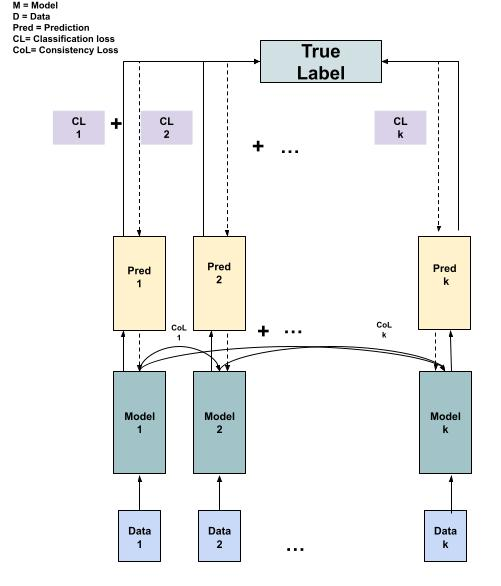
\includegraphics[width=1\linewidth]{mainmatter/emnlp2021_gl/multiple_students_architecture.jpeg}
\caption{ The multiple-student architecture for knowledge distillation.}
\label{multiple_students_architecture}
\vspace{-7mm}
\end{figure}
\subsection{Model Distillation}

%To mitigate the risk that a chosen data distillation technique might be overly aggressive, we propose a combined distillation strategy. Specifically, we introduce a \textit{Group Learning} architecture (shown in figure), inspired from the teacher-student paradigm \cite{hinton2015distilling,tarvainen2017mean,laine2016temporal,sajjadi2016regularization}. In this architecture each student method is trained on two techniques.
To mitigate the risk of distilling the data at the incorrect granularity (overly aggressive or too conservative), we propose a combined distillation strategy. Specifically, we introduce a \textit{Group Learning} architecture (shown in Figure~\ref{multiple_students_architecture}), inspired from the teacher-student paradigm \cite{hinton2015distilling,tarvainen2017mean,laine2016temporal,sajjadi2016regularization}. In this architecture each student method is trained on two techniques:

{\flushleft (a)} Different versions of the same dataset, each delexicalized differently by using different data distillation techniques mentioned above.

{\flushleft (b)} The distributions of predictions of other models.

This combined methodology of knowledge distillation encourages students to learn as much as possible from their own views of the data, while jointly learning with other students. Training together on the soft labels (distribution of predictions) of other student methods  acts as a form of regularization between all methods.
%, but  each student model is also thus encouraged to extract transferable facts from a given fact verification dataset. % ms: BS
More formally, each student component includes a regular classification loss (implemented using cross entropy) on their respective data. Additionally, they each have a consistency loss between all other methods that minimizes the difference in predicted label distributions between them.

The intuition behind our approach is that by providing multiple data distillation options to choose from we encourage the student methods to `pull' towards each other and the original underlying semantics. The part of semantic knowledge that is obscured from a student method due to the particular delexicalization technique used in the dataset version it sees, is instead learned in its effort to perform on par with other methods.
Thus, similar to a classroom environment where the students learn from both, known labels (e.g., a textbook) and by helping another student learn, each student is able to thus choose the right amount of granularity needed to enhance its own understanding.

\section{Models and Data}

\textbf{Models:} Since it had achieved state-of-the art results in many NLP tasks, including fact verification, BERT \citep{devlin-etal-2019-bert} 
%(with transformer networks \citep{vaswani2017attention} as the underlying classifier) 
was our  choice for the pre-trained model used in our experiments. We experiment with two variants, BERT-Base, and Mini BERT \cite {turc2019well}, a light-weight version of BERT, both from the Hugging Face repository \citep{wolf2019huggingface}.
\textbf{Data:} We use two distinct fact verification datasets for
our experiments,The Fact Extraction and Verification (FEVER) dataset  \citep{thorne-etal-2018-fact} and the Fake News Challenge (FNC) dataset \citep{pomerleau2017fake}.

The FEVER dataset consists of 145,449 data points each having a claim and evidence pair. These claim-evidence pairs typically contain one or more sentences compiled from Wikipedia using an information retrieval (IR) module and are classified into three classes: \textit{supports, refutes} and \textit{not enough info}. The evidence for data points that had the gold label of \textit{not enough info} were  retrieved (using a task-provided IR component) either by finding the nearest neighbor to the claim or randomly. Even though the training partition of the FEVER dataset was publicly released, the gold test labels used in the final shared task were not. We therefore built our own test partition by dividing the randomized training partition into 80\% (119,197 data points) and 20\% (26,252 data points).

The FNC dataset comprises claim-evidence pairs that were divided into four classes, \textit{agree, disagree, discuss} and \textit{unrelated}. These claim-evidence pairs were created using the headlines and content section of real news articles respectively. While the training partition of the publicly available dataset comprised of 49,972 data points, the testing partition had 25,413 data points. We further divided the training partition into
40,904 data points for training and 9,068 data points for development.

In order to evaluate the proposed methods in a cross-domain setting, we modified the label space of the source domain to match that of the target domain as done in previous chapters.

\section{Experiments}
In all the experiments, the performance of the underlying method on the respective original, lexicalized data is considered as the baseline. In the baseline model, we use the default hyper parameters from Hugging Face. 
We focus our analysis on cross-domain evaluation, i.e., we train all methods on one dataset  (e.g., FEVER) and evaluate their accuracy on the other dataset (e.g., FNC). At the end of training, the best student model from the list of all the trained models is saved to be used for evaluation.



\begin{table}[h]
\begin{center}
\footnotesize
\begin{tabular}{p{20mm}p{9mm}p{9mm}|p{9mm}p{9mm}}
\toprule
& \multicolumn{4}{c}{Configuration} \\
\midrule
Train  & {FEVER}&{FEVER}&{FNC}&{{FNC}} \\
Eval  & {FEVER}&{{FNC}}&{FNC}&{{FEVER}} \\
\midrule
Mini BERT Lex &83.86\%&69.50\%&89.33\%&54.11\%\\
Mini BERT \bf{GL} &83.74\%&{73.06\%*}&89.72\%&{74.46\%*}\\
\midrule
BERT-Base Cased Lex&90.88\%&66.68\%&90.88\%&73.78\%\\
BERT-Base Cased \bf{GL}&84.88\%&{\textbf{75.37}\%*}&87.07\%&75.51\%\\
\midrule
BERT-Base Uncased Lex&91.95\%&64.21\%&91.95\%&76.59\%\\
BERT-Base Uncased \bf{GL} &86.12\%&{73.61\%*}&98.42\%&\textbf{77.67\%}\\

\bottomrule
\end{tabular}
\end{center}
\caption{ In-domain and cross-domain accuracies for various methods.
All scores reported are averaged across three random seeds.
``Lex'' is the stand alone model trained on the original lexicalized data;  ``GL'' denotes the student in the proposed multi-student `Group Learning' architecture. * indicates that the corresponding result is significantly better than its baseline (``lex'' in the same column), under a bootstrap resampling test with 1,000 samples, and $p$-value $< 0.05$. }
\label{results_fnc}
\vspace*{-5mm}
\end{table}

\section{Results}
Table \ref{results_fnc} summarizes our results. We focus on two sets of experiments using each training method and setting: in-domain (columns 2 and 4) and cross-domain (columns 3 and 5).
Although all models perform well (83.86\%--99.5\%) in-domain, they transfer poorly when evaluated cross-domain where up to 35\% drop in performance is observed. This verifies our findings that the signal the model learns from un-masked text does not generalize well between domains.
On the other hand, we observe a marginal in-domain drop in performance for the student models trained on the GL architecture (e.g., 9.5\% in the FEVER/FEVER setting for BERT-Base Cased) compared to their lexical counter parts. This indicates that GL models retain most signal from lexical data. Importantly, the GL models perform considerably better than their corresponding lexical versions across domain (e.g., up to 20.36\% improvement in the FNC/FEVER setting for Mini-BERT). This demonstrates that data distillation and model distillation can be successfully combined as a strategy to improve domain transfer of fact verification methods.
%\mihaiCheck{From Sandeep: Should I keep it high level like this, or talk about each model's numbers?, Thanks.} % ms: this is Ok

%\begin{table}[t]
%\begin{center}
%\footnotesize
%\begin{tabular}{p{10mm}|p{12mm}p{12mm}p{12mm}}
%\midrule
%& \multicolumn{3}{c}{Best Student} \\
%\midrule
%Fever to FNC &Lex&Lex&FIGER Specific\\
%\midrule
%FNC to Fever &FIGER Abstract&OA NER&OA NER\\
%\bottomrule
%\end{tabular}
%\end{center}
%\caption{\label{crossdomain} Type of model (out of the 4 students that were trained together) that performed best in the two cross-domain experiments, %for three random seeds.}
%\label{random_seed_expts}
%\vspace*{-5mm}
%\end{table}

\section{Discussion and Conclusion}
Previous work has shown that delexicalization is useful in learning domain transferable knowledge. However, the level of delexicalization suitable for each task is unclear. In this work, we provide multiple delexicalization choices to neural network models and encourage them to choose the most appropriate choice.
We suspect this approach acts as regularization (through the consistency losses), as well as a form of data noise (because of the imperfect NERs), which has been shown to aid in knowledge distillation paradigms \citep{hinton2015distilling,tarvainen2017mean}.

%\mihaiCheck{Should we keep or delete this?-->} Further, in Table ~\ref{random_seed_expts} we show which particular method (out of the students that were trained together), performed best in each scenario according to accuracy on cross-domain development partition (for 3 different random seeds). 
Further, analyzing the selection made by the GL framework for various random seeds, we observed that when trained on FEVER and tested on FNC, GL selects the lexicalized student, while in the other cross-domain direction the common choice is the student delexicalized with OA-NER. 
%For the first direction, trained on FEVER and tested on FNC, two out of the three best classifiers were students trained on the lexicalized, plain-text FEVER dataset. However, in the case of the second direction, i.e., trained in FNC and tested on FEVER, the best performers were students whose datasets were delexicalized with either FIGER Abstract or  OA-NER. 
We hypothesize this happens for two reasons. First, the training data in the FNC dataset is smaller (40,904 data points) when compared to that of the FEVER dataset (119,197 training data points), so it is more prone to overfitting in the original, lexicalized form. Second, since the FNC dataset is derived from real-world news articles, the number of evidence sentences in the FNC are higher than the sentences in FEVER. This means that delexicalized sentences in FNC preserve enough lexical signal for training, even in their delexicalized forms. The opposite observations hold in the other direction (FEVER to FNC), which caused the lexicalized students to perform better. 
Also do note that even though we use only 4 student methods  in our experiments to train with  each other, this can be extended to any number of methods. However, the right number of student models (and their corresponding delexicalized datasets) for a given task needs to be empirically determined. 

Our approach demonstrates that: (a) delexicalization helps model generalization, (b) the amount of delexicalization to apply varies from dataset to dataset, and (c) it is possible to learn how much delexicalization to apply through our proposed GL architecture.


